\chapter{Практическая часть} \label{ch2}
	
% не рекомендуется использовать отдельную section <<введение>> после лета 2020 года
%\section{Введение} \label{ch2:intro}

\section{Используемые инструменты} \label{ch2:title-abbr} %название по-русски
	Для реализации был выбран язык программирования Python 3.9. Среда разработки: JetBrains PyCharm.
	Также, использовались такие пакеты для языка Python, как: 
\begin{itemize}
	\item math, numpy - для расчетов;
	\item scipy - для работы с wav-файлом.
\end{itemize}

Для работы с гармоническими процессами использовались ранее реализованные в рамках курса \cite{bel} функции библиотеки spbstu-processing-data. 

\section{Модели и константы}

Для работы с данными генерируемых сигналов был создан класс Signal, который хранит в себе значения сигнала, частоту дискретизации и интерпретируемый символ.

Значения частот, соответствующих символов приведены в программе в виде констант:
\begin{itemize}
	\item DTMF\_TABLE - словарь символов и частот;
	\item DTMF\_FREQ - массив возможных частот набора;
	\item DTMF\_HIGH - массив высоких частот;
	\item DTMF\_LOW - массив низких частот.
\end{itemize}

\section{Чтение и запись}

Чтобы записывать значения сигналов в файл был создан класс Writer, который в функции \textit{def write(filename: str, signals: [Signal])} формирует из объектов Signal весь массив значений и передает его на вход функции \textit{write} библиотеки scipy.

Для чтения данных из wav-файла используется класс Reader и функция \textit{def read(filename: str)}, которая обращается к \textit{read} фреймворка scipy.

\section{Генерация сигнала}

Чтобы создать звуковой файл, был написан класс Generator, в котором реализованы две функции:

\begin{itemize}
	\item \textit{def generate\_from(symbols: str, duration, volume, rate) → [Signal]} - принимает на вход строку символов с заданными параметрами продолжительности, громкости и частоты и возвращает массив сгенерированных элементов Signal;
	\item \textit{def calculate(symbol: str, duration, volume, rate) → Signal} - для входного символа вычисляет значение двух гармоник и их аддитивную модель.
\end{itemize}

Результат функции \textit{generate\_from} передается объекту класса Writer, описанному ранее.

\section{Распознавание символов}

Алгоритм Гёрцеля реализован в рамках класса Goertzel, в котором используются следующие функции и методы:

\begin{itemize}
	\item \textit{init} - инициализатор класса, в котором заранее подсчитываются значения коэффициентов DTMF-частот;
	\item \textit{def calc\_s\_n(self, sample\_data)} - вычисляет значения последовательности $s_n$;
	\item \textit{def calc\_power(self) -> \{float: float\}} - вычисляет мощность для каждого частотного компонента;
	\item \textit{def get\_number(self, powers)} - на основе полученных мощностей находим необходимый нам символ по таблице DTMF\_TABLE;
	\item \textit{def reset(self)} - для каждого последующего пакета значений сигнала сбрасываем посчитанные значения последовательности $s_n$.
\end{itemize}

Чтобы определить символы, которые были закодированы в wav-файле, был определен класс Detector. Он включает в себя одну функцию:

\begin{itemize}
	\item \textit{def detect(rate, data) -> str} - принимает на вход частоту и значения сигнала, а возвращает строку с распознанным сообщением.
\end{itemize}

В рамках этапа распознавания разбиваем массив значений сигнала на пакеты (bins), элементы которых поочередно передаем на вход алгоритма Гёрцеля - объекту класса Goertzel. В итоге получаем строку распознанных значений.

\section{Пример работы генерации сигнала}

Результатом работы является wav-файл, который можно прослушать по данной ссылке. Спектрограмма сигнала для сообщения $"147*"$ на \firef{fig:step-9}.

\begin{figure}[ht] 
	\center
	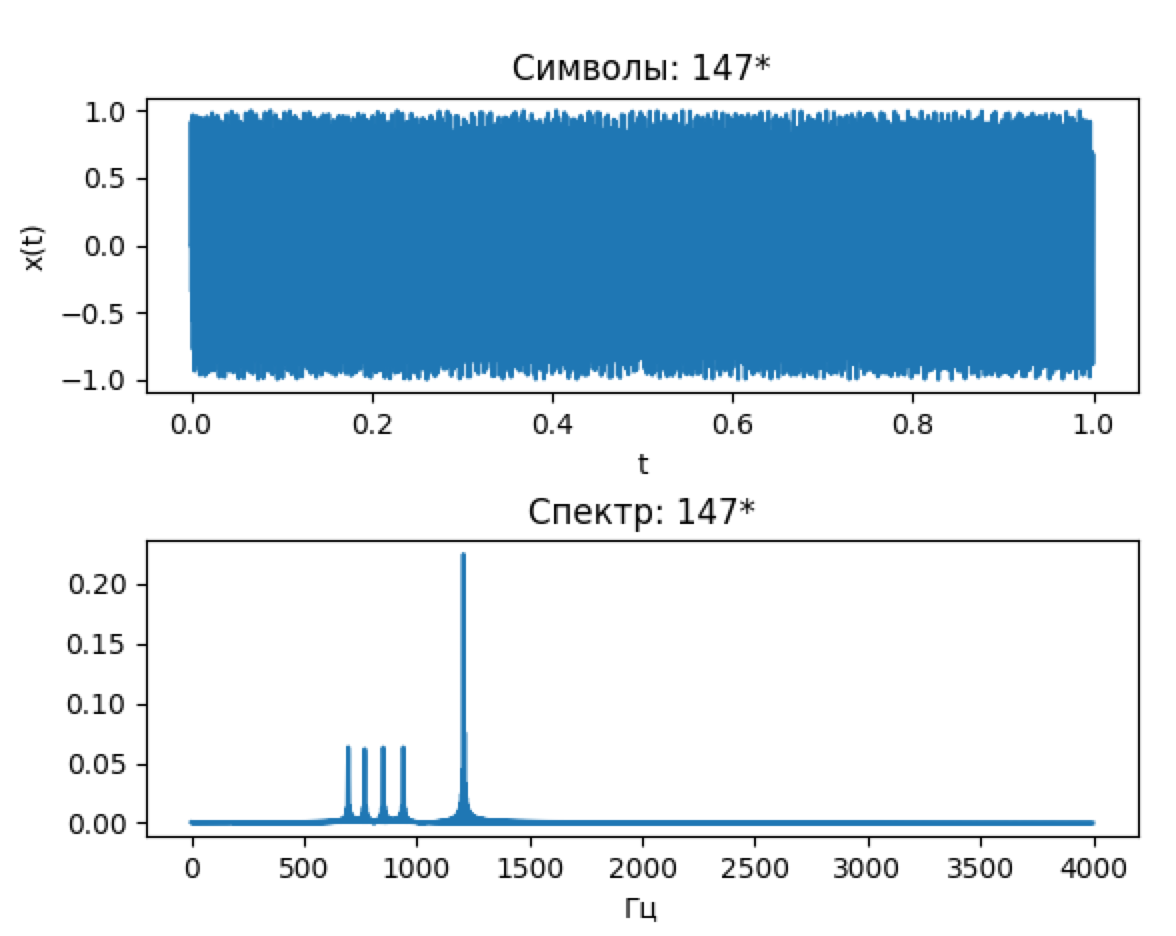
\includegraphics [scale=0.7] {my_folder/images/step-9}
	\caption{Спектрограмма сигнала сообщения $"147*"$} 
	\label{fig:step-9}
	\end{figure}

\section{Пример работы декодирования сигнала}

Результатом работы детектирования является строка с распознанным текстом, который можно удобно распечатать, как показано на 

\begin{figure}[ht] 
	\center
	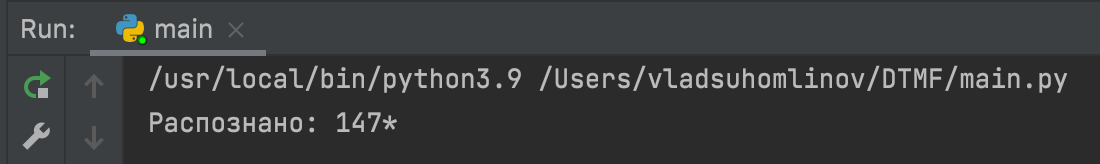
\includegraphics [scale=0.7] {my_folder/images/step-8}
	\caption{Вывод сообщения о распознанном сигнале} 
	\label{fig:step-8}
	\end{figure}

Теперь необходимо обратимо обратиться к проблеме шума. Не исключено, что при передаче аудио-сигнал может искажаться случайным шумом.

При небольшом шуме, превышающий исходный сигнал по амплитуде исходный в 2 раза, для сообщения $"147*"$ мы можем уверенно распознать необходимые нам частоты благодаря спектру Фурье \cite{book}, как показано на \firef{fig:step-6}:

\begin{figure}[ht] 
	\center
	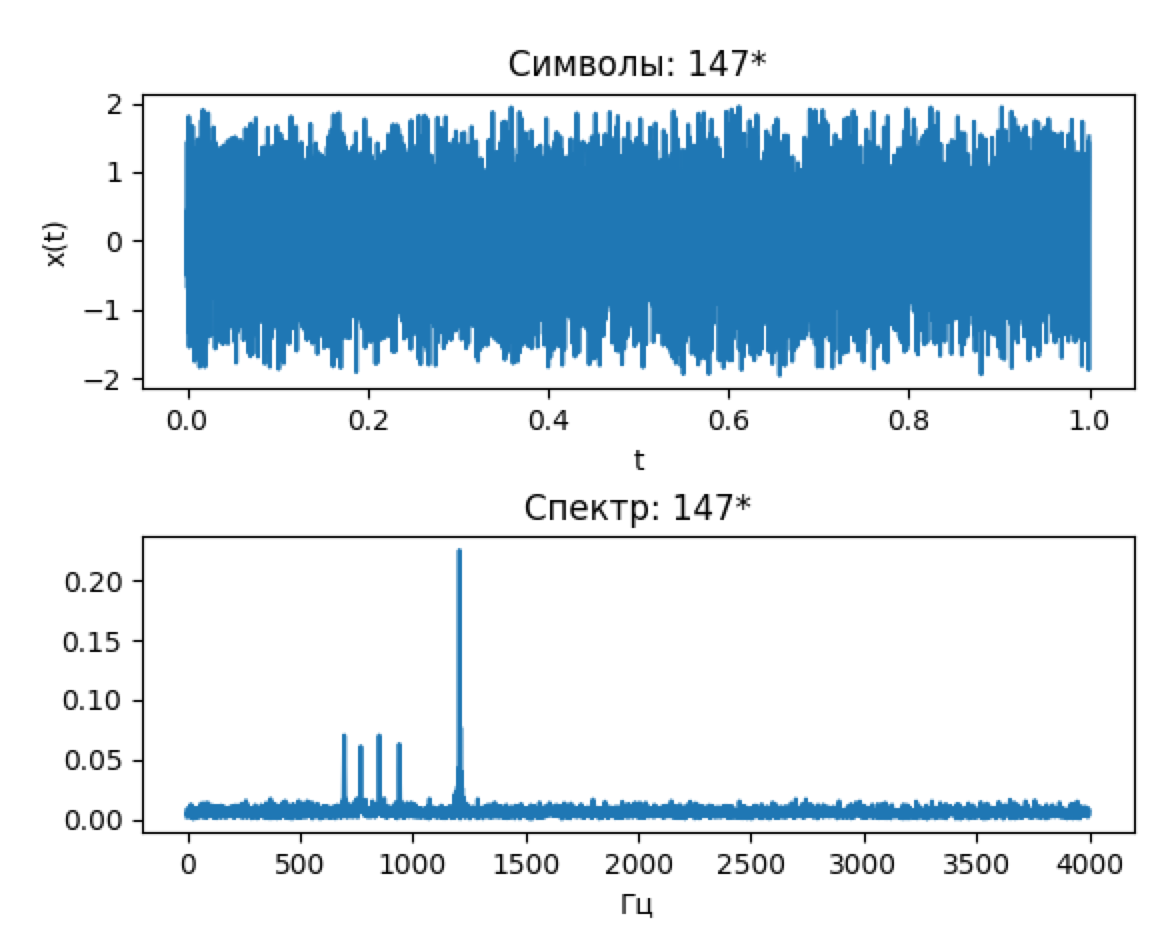
\includegraphics [scale=0.7] {my_folder/images/step-6}
	\caption{Результат применения шума к сигналу} 
	\label{fig:step-6}
	\end{figure}
	
Дополнительное применение полосового фильтра BSW \cite{bel} со значением m равным 64 позволяет улучшить работу декодирования в тех случаях, когда шум превышает исходный сигнал в 5 раз (\firef{fig:noize}).

\begin{figure}[ht] 
	\center
	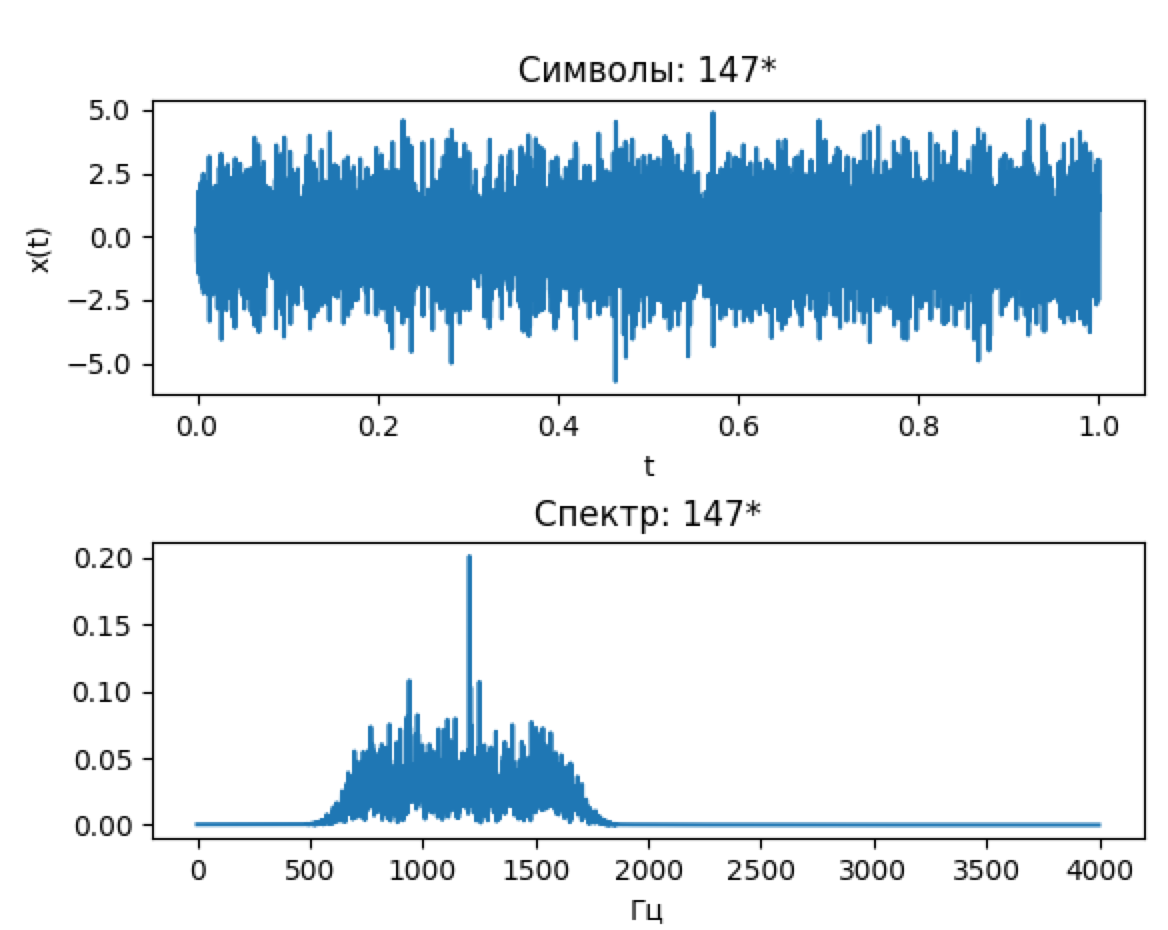
\includegraphics [scale=0.7] {my_folder/images/noize}
	\caption{Применение полосового фильтра для улучшения разпознавания} 
	\label{fig:noize}
	\end{figure}

\section{Выводы} \label{ch2:conclusion}

В результате работы удалось реализовать инструменты для работы с звуковыми данными, успешно закодирован алгоритм Гёрцеля и проверена работа распознавания с шумом и без.


%% Вспомогательные команды - Additional commands
%
\newpage % принудительное начало с новой страницы, использовать только в конце раздела
%\clearpage % осуществляется пакетом <<placeins>> в пределах секций
\newpage\leavevmode\thispagestyle{empty}\newpage % 100 % начало новой страницы